\documentclass[a4paper,openright,12pt]{report}
\usepackage[spanish]{babel} 
\usepackage[latin1]{inputenc} 
\usepackage{graphicx}
\graphicspath{{images/pdf/}}
\usepackage{cite} % para contraer referencias
\usepackage{url} 
\begin{document}
\chapter{Marco Conceptual}
Este capitulo pretende definir todos los conceptos vinculados con el desarrollo del proyecto, en los aspectos de gobernanza en SOA, versionados y calidad de servicios.
\section{Gobernanza en SOA}
\section{Versionado de Servicios}
\section{Calidad de Servicios}
La calidad de los servicios es un elemento importante que permite determinar la facilidad de uso, utilidad y rendimiento del servicio entre otros factores.
\subsection{Metamodelo de calidad}
Un metamodelo de calidad permite definir distintos niveles para evaluar la calidad de un servicio. El metamodelo basico es "Quality Abstract" que contiene la siguiente estructura
\begin{figure} [h]
\centering
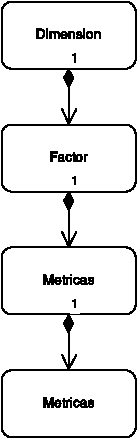
\includegraphics[width=1\textwidth]{images/pdf/metamodelo_de_calidad.pdf}
	\caption{Niveles del Metamodelo de Calidad Absrtacto}
  	\label{figura:metamodelo_de_calidad}
\end{figure}

La figura \ref{figura:metamodelo_de_calidad} nos indican los siguientes niveles:


\bibliographystyle{acm}
\bibliography{biblio}
\end{document}
